% analysis.tex

\chapter{Analysis}
\thispagestyle{chapterstart}

\section{Methodology}

In this section, we refine our evaluation criteria for side-channel resistant implementations of \ac{PQC} schemes by incorporating detailed analyses from recent literature. We focus on masking techniques, performance metrics, and practicality on embedded devices, drawing from specific methodologies used in studies such as Migliore et al.\ (2019) \cite{Migliore19}.

Our evaluation criteria are:

\begin{itemize}
    \item \textbf{Side-Channel Resistance Evaluation:} The methodologies employed to assess side-channel vulnerabilities, including the use of Welch's t-test, single-bit Differential Power Analysis (DPA), and Test Vector Leakage Assessment (TVLA), as demonstrated in Migliore et al.\ (2019) \cite{Migliore19} and Heinz et al.\ (2020) \cite{Heinz20}.
    \item \textbf{Masking Techniques:} The specific masking strategies applied, such as Boolean masking, arithmetic masking, or hybrid approaches, and their effectiveness in preventing side-channel leakage. We consider the order of masking and the associated security proofs in the probing model \cite{Migliore19}.
    \item \textbf{Implementation Efficiency:} The computational overhead introduced by masking, including execution time, memory usage, and the impact on performance-critical operations like polynomial multiplication and decomposition. Metrics are drawn from implementation results reported in studies like Migliore et al.\ (2019) \cite{Migliore19} and Bronchain and Cassiers (2022) \cite{Bronchain22}.
    \item \textbf{Algorithmic Modifications for Efficiency:} Any algorithmic changes proposed to enhance masking efficiency, such as modifying the modulus to a power of two \cite{Migliore19}, and their implications for security and performance.
    \item \textbf{Practicality and Scalability:} The feasibility of implementing the proposed countermeasures on resource-constrained embedded devices, including considerations for assembly-level optimizations and hardware-specific challenges.
\end{itemize}

Using these refined criteria, we will perform an in-depth analysis of the selected implementations, emphasizing how each addresses the challenges of side-channel resistance in \ac{PQC} schemes.

\section{In-Depth Analysis of Selected Implementations}

\subsection{Migliore et al.\ (2019): Masking Dilithium for Side-Channel Resistance}

Migliore et al.\ \cite{Migliore19} present one of the first comprehensive studies on masking the Dilithium signature scheme to protect against side-channel attacks. Their work focuses on evaluating the side-channel leakage of an unprotected implementation of Dilithium and proposing efficient masking techniques to mitigate these vulnerabilities.

\subsubsection{Side-Channel Evaluation of Unmasked Dilithium}

The authors first perform a side-channel analysis of an unmasked implementation of Dilithium on an ARM Cortex-M3 microcontroller (STM32F1). They target critical functions such as \texttt{LowBits\_q}, \texttt{HighBits\_q}, and rejection sampling operations, which are susceptible to side-channel leakage due to their manipulation of secret-dependent data.

Using Welch's t-test and single-bit DPA on the electromagnetic (EM) emissions, they demonstrate that significant leakage occurs in these functions with as few as 500 traces. As illustrated in Figure~\ref{fig:dpa_curves}, the single-bit DPA curves for the \texttt{Rejection}, \texttt{LowBits\_q}, and \texttt{HighBits\_q} functions reveal clear peaks, indicating exploitable leakage.

\begin{figure}[h]
    \centering
    \begin{subfigure}[b]{0.3\textwidth}
        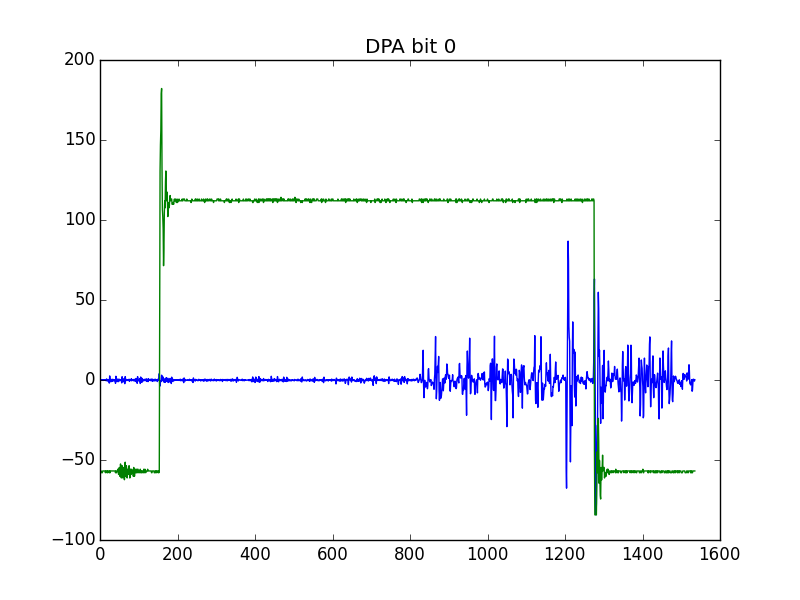
\includegraphics[width=\textwidth]{../figures/Rejection.png}
        \caption{\texttt{Rejection}}
        \label{fig:rejection}
    \end{subfigure}
    \hfill
    \begin{subfigure}[b]{0.3\textwidth}
        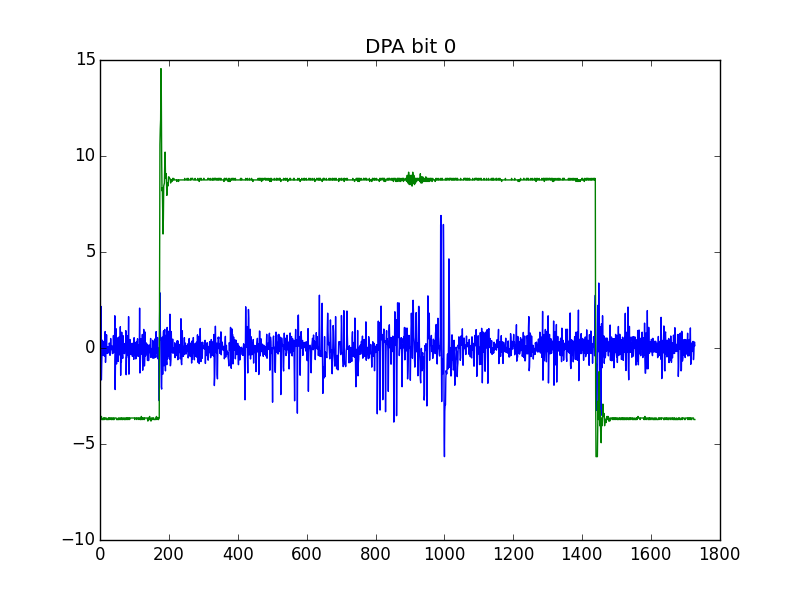
\includegraphics[width=\textwidth]{../figures/LowBits.png}
        \caption{\texttt{LowBits\_q}}
        \label{fig:lowbits}
    \end{subfigure}
    \hfill
    \begin{subfigure}[b]{0.3\textwidth}
        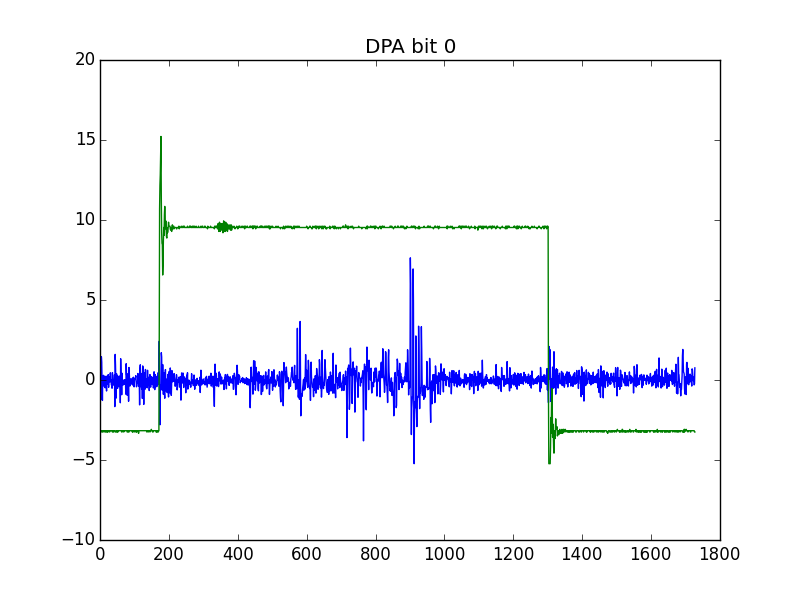
\includegraphics[width=\textwidth]{../figures/HighBits.png}
        \caption{\texttt{HighBits\_q}}
        \label{fig:highbits}
    \end{subfigure}
    \caption{Single-bit DPA curves on bit 0 of sensitive data (using 500 traces). Significant peaks indicate leakage in unmasked implementations.}
    \label{fig:dpa_curves}
\end{figure}

This evaluation underscores the necessity of implementing countermeasures to protect Dilithium against side-channel attacks on embedded devices.

\subsubsection{Algorithmic Modification: Power-of-Two Modulus}

A significant innovation in their work is the proposal to modify the modulus $q$ from a prime number to a power of two. This change simplifies the masking of certain operations, particularly the decomposition functions like \texttt{HighBits\_q} and \texttt{LowBits\_q}, which become straightforward bit-shifting operations when $q$ is a power of two.

This modification results in considerable performance improvements, achieving speedups of up to $8\times$ for the most time-consuming masking operations, as shown in Table~\ref{tab:performance-masking}.

\begin{table}[h]
    \centering
    \caption{Execution times of main gadgets for both prime and power-of-two modulus $q$ on STM32F1 (order-1 masking, computation on 1 coefficient).}
    \label{tab:performance-masking}
    \begin{tabular}{|l|c|c|c|}
        \hline
                                           & $q = 8380417$              & $q = 2^b$                & Speedup   \\
        \hline
        \texttt{arith::to::bool::lowbits}  & 331 $\mu$s / 7,944 cycles  & 38 $\mu$s / 912 cycles   & $8\times$ \\
        \texttt{arith::to::bool::highbits} & 275 $\mu$s / 6,600 cycles  & 37 $\mu$s / 888 cycles   & $7\times$ \\
        \texttt{arith::makehint}           & 560 $\mu$s / 13,440 cycles & 79 $\mu$s / 1,896 cycles & $7\times$ \\
        \texttt{bool::rejection}           & 66 $\mu$s / 1,584 cycles   & 66 $\mu$s / 1,584 cycles & $1\times$ \\
        \hline
    \end{tabular}
\end{table}

They argue that this alteration does not affect the security of the scheme, relying on a modulus-switching argument to maintain the hardness of the underlying lattice problems.

\subsubsection{Performance Overhead of Masking}

To quantify the performance impact of the proposed masking techniques, Migliore et al.\ measured the execution times for \texttt{DILITHIUM.KeyGen} and \texttt{DILITHIUM.Sign} operations with different masking orders. As presented in Table~\ref{tab:overall-performance}, the first-order masked implementation incurs a performance overhead of approximately $5.6\times$ compared to the unmasked version for both key generation and signature operations.

\begin{table}[h]
    \centering
    \caption{Execution times of \texttt{DILITHIUM.KeyGen} and \texttt{DILITHIUM.Sign} on an Intel Core i7-7600U CPU running at 2.80 GHz (10,000 runs).}
    \label{tab:overall-performance}
    \begin{tabular}{|l|c|c|c|c|}
        \hline
                        & No Masking           & Order-1 Masking & Order-2 Masking & Order-3 Masking \\
        \hline
        \texttt{KeyGen} & 323 $\mu$s           & 1.83 ms         & 2.52 ms         & 4.32 ms         \\
                        & (\textit{reference}) & ($5.66\times$)  & ($7.8\times$)   & ($13.4\times$)  \\
        \hline
        \texttt{Sign}   & 992 $\mu$s           & 5.64 ms         & 11.68 ms        & 28.08 ms        \\
                        & (\textit{reference}) & ($5.68\times$)  & ($11.77\times$) & ($28.3\times$)  \\
        \hline
    \end{tabular}
\end{table}

\subsubsection{Side-Channel Resistance Evaluation of Masked Dilithium}

To demonstrate the effectiveness of their masking techniques, the authors performed a t-test analysis using 10,000 traces. Figure~\ref{fig:t-test-masked} illustrates the evaluation results, showing no detectable first-order leakage in the masked implementation, as all t-values remain within the $\pm4.5$ threshold. This contrasts with the unmasked version, where significant leakage was detected with only 500 traces (see Figure~\ref{fig:dpa_curves}).

\begin{figure}[h]
    \centering
    \begin{subfigure}[b]{0.45\textwidth}
        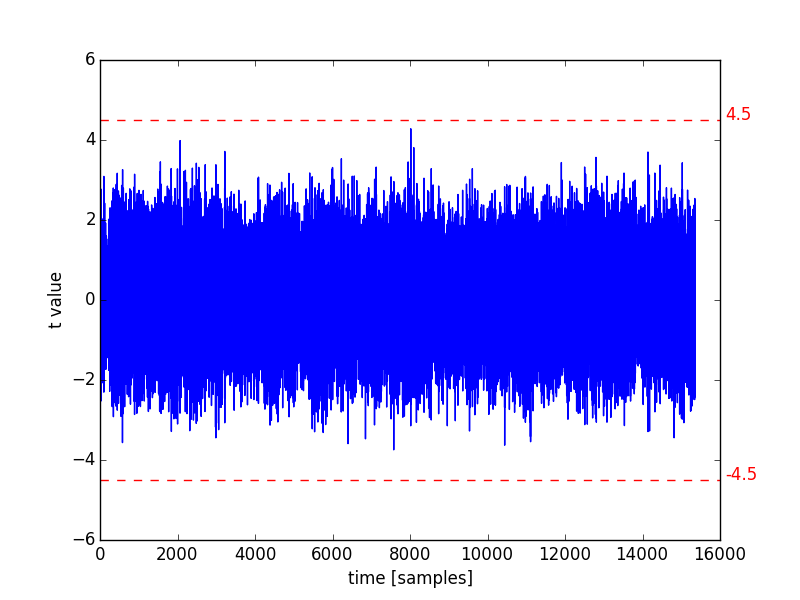
\includegraphics[width=\textwidth]{../figures/bool_rejection_10000_traces.png}
        \caption{\texttt{bool::rejection}}
        \label{fig:bool_rejection}
    \end{subfigure}
    \hfill
    \begin{subfigure}[b]{0.45\textwidth}
        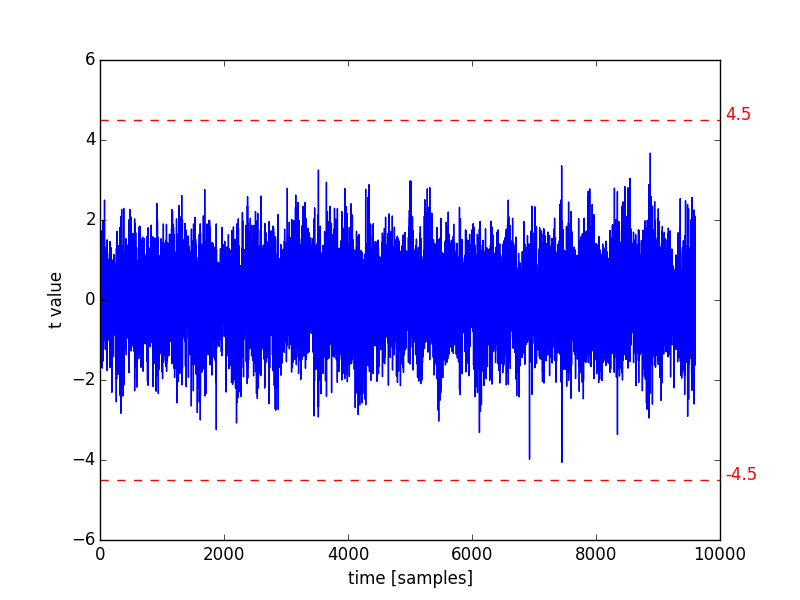
\includegraphics[width=\textwidth]{../figures/arith_to_bool_lowbits_10000_traces.png}
        \caption{\texttt{arith::to::bool::lowbits}}
        \label{fig:arith_to_bool_lowbits}
    \end{subfigure}
    \vfill
    \begin{subfigure}[b]{0.45\textwidth}
        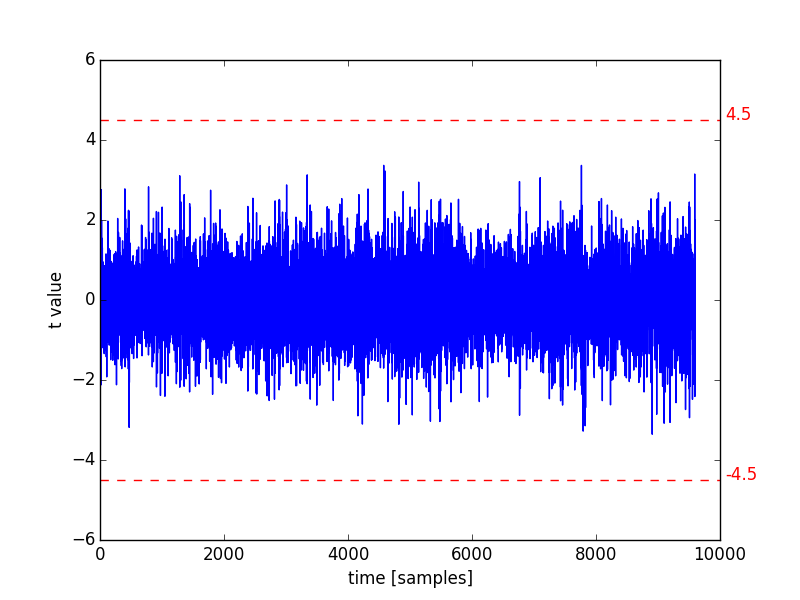
\includegraphics[width=\textwidth]{../figures/arith_to_bool_highbits_10000_traces.png}
        \caption{\texttt{arith::to::bool::highbits}}
        \label{fig:arith_to_bool_highbits}
    \end{subfigure}
    \hfill
    \begin{subfigure}[b]{0.45\textwidth}
        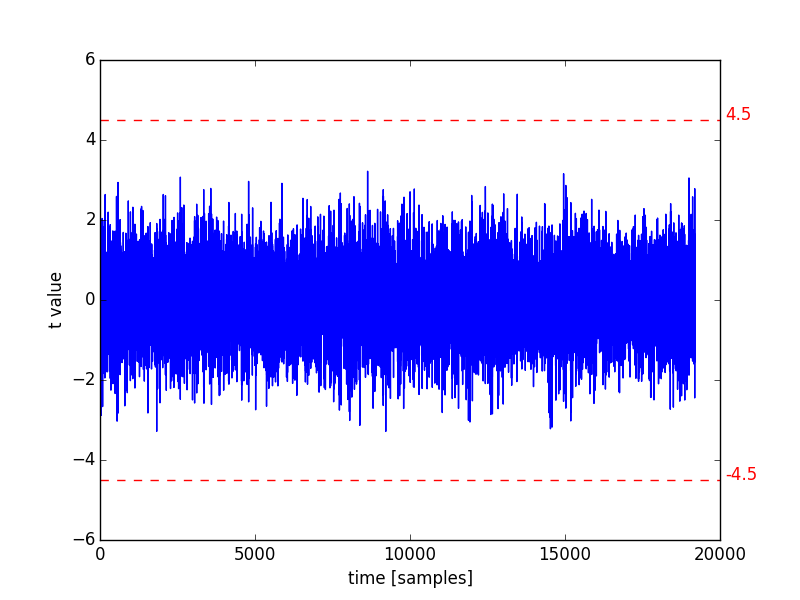
\includegraphics[width=\textwidth]{../figures/arith_makehint_10000_traces.png}
        \caption{\texttt{arith::makehint}}
        \label{fig:arith_makehint}
    \end{subfigure}
    \caption{Evaluation of the Welch's t-test on masked gadgets after 10,000 traces. The t-values remain within the $\pm4.5$ threshold, indicating no detectable first-order leakage.}
    \label{fig:t-test-masked}
\end{figure}

\subsubsection{Discussion of Trade-offs}

While the masking techniques significantly improve side-channel resistance, they introduce computational overhead. The use of a power-of-two modulus mitigates some of this overhead but may have implications for compatibility and standardization, as the original Dilithium specification uses a prime modulus. The trade-off between security and performance must be carefully considered, especially for resource-constrained embedded devices.

% \subsubsection{Metrics for Comparison}

% Key metrics from Migliore et al.\ (2019) that can be used for comparison include:

% \begin{itemize}
%     \item \textbf{Execution Time:} Measured in cycles or microseconds for key operations before and after masking.
%     \item \textbf{Performance Overhead Factors:} Quantitative factors indicating how much slower the masked implementation is compared to the unmasked version (e.g., $5.6\times$ for first-order masking).
%     \item \textbf{Side-Channel Leakage Evaluation Results:} Number of traces required to detect leakage in unmasked versus masked implementations.
%     \item \textbf{Speedup Achieved with Power-of-Two Modulus:} Performance gains in masking operations due to the modulus modification (e.g., $7\times$ to $8\times$ speedup).
% \end{itemize}

% These metrics can be incorporated into tables and figures to visually compare the effectiveness and efficiency of side-channel countermeasures across different implementations.

\subsection{Heinz et al.\ (2020): First-Order Masked Kyber on ARM Cortex-M4}

[To be done]

\subsection{Bos et al.\ (2021): Higher-Order Masking for Kyber}

[To be done]

\subsection{Coron et al.\ (2023): Improved Masking Gadgets for Dilithium}

[To be done]

\subsection{Bronchain and Cassiers (2022): Bitslicing Techniques for Lattice-Based KEMs}

[To be done]

\section{Comparative Analysis}

Based on the in-depth analyses, we can compare the implementations across our evaluation criteria:

\begin{itemize}
    \item \textbf{Masking Techniques:} Migliore et al.\ (2019) focus on masking Dilithium using both Boolean and arithmetic masking, introducing specific masked gadgets and modifying the modulus for efficiency. Other works like Heinz et al.\ (2020) and Bos et al.\ (2021) also employ masking but focus on Kyber.
    \item \textbf{Performance Metrics:} The overhead introduced by masking varies among implementations. Migliore et al.\ report a $5.6\times$ overhead for first-order masking, while Bronchain and Cassiers (2022) achieve up to $1.8\times$ speedup using bitslicing techniques.
    \item \textbf{Side-Channel Resistance Evaluation:} All implementations validate their side-channel resistance using methods like TVLA or DPA. Migliore et al.\ demonstrate that their masked implementation resists leakage detection even after 10,000 traces.
    \item \textbf{Algorithmic Modifications:} Migliore et al.\ uniquely propose modifying the modulus to a power of two, whereas others focus on optimizing existing algorithms.
    \item \textbf{Practicality and Scalability:} The feasibility of these implementations on embedded devices varies, with some requiring significant resources due to higher-order masking or complex gadgets.
\end{itemize}

We can visualize these comparisons in tables and graphs, highlighting the trade-offs between security and efficiency in each approach.

% Include any additional figures or tables here as needed.

% Remember to reference the figures and tables in the text.

